% Document type, global settings, and packages

\documentclass[12pt]{report}   %12 point font for Times New Roman
\usepackage{graphicx}  %for images and plots
\usepackage[letterpaper, left=1in, right=1in, top=1in, bottom=1in]{geometry}
\usepackage{setspace}  %use this package to set linespacing as desired
\usepackage{times}  %set Times New Roman as the font
\usepackage[explicit]{titlesec}  %title control and formatting
\usepackage[titles]{tocloft}  %table of contents control and formatting
\usepackage[backend=bibtex, sorting=none, bibstyle=ieee, style=numeric]{biblatex}  %reference manager
\usepackage{appendix}  %for appendices
\usepackage{rotating}  %for rotated, landscape images
\usepackage[normalem]{ulem}  %for underlined section titles
\usepackage{textcomp} % for text symbols such as copyright etc. 
\usepackage{indentfirst} % To indent the first line of every paragraph
\usepackage{booktabs,array,arydshln} %for better table formatting. 
\usepackage{amsmath} %for formula formatting
\usepackage{ amssymb }
\usepackage{gensymb}
\usepackage[T1]{fontenc} % improved font encoding
\usepackage[utf8]{inputenc} % for better handling of non-ASCII characters
%\usepackage{newtxtext} % font choice
\usepackage{newtxmath} 
%\usepackage{lmodern} % font choice 
%\usepackage[bookmarks=true, hidelinks]{hyperref}
\usepackage[hidelinks]{hyperref}
\usepackage{physics}


% Bibliography
%Add your bibliography file here
\bibliography{references}

% prevent certain fields in references from printing in bibliography
\AtEveryBibitem{\clearfield{issn}}
\AtEveryBibitem{\clearlist{issn}}

\AtEveryBibitem{\clearfield{language}}
\AtEveryBibitem{\clearlist{language}}

\AtEveryBibitem{\clearfield{doi}}
\AtEveryBibitem{\clearlist{doi}}

\AtEveryBibitem{\clearfield{url}}
\AtEveryBibitem{\clearlist{url}}

\AtEveryBibitem{%
  \ifentrytype{online}
    {}
    {\clearfield{urlyear}\clearfield{urlmonth}\clearfield{urlday}}}


% Start of Dissertation Document

\begin{document}
\doublespacing  %set line spacing to double by default through out the document. This can be overwritten when necessary

% Title Page (No page number)
%This is the tile page of your dissertation
%Please type below title of your dissertation and your name
%change the year if neccessary

\begin{titlepage}
\begin{center}

\begin{singlespacing}
\vspace*{6\baselineskip}
[ATLAS Semivisible Jets]\\
\vspace{3\baselineskip}
[Elena Laura Busch]\\
\vspace{18\baselineskip}
Submitted in partial fulfillment of the\\
requirements for the degree of\\
Doctor of Philosophy\\
under the Executive Committee\\
of the Graduate School of Arts and Sciences\\
\vspace{3\baselineskip}
COLUMBIA UNIVERSITY\\
\vspace{3\baselineskip}
\the\year
\vfill


\end{singlespacing}

\end{center}
\end{titlepage}





% Copyright  Page (No page number)


\begin{titlepage}
\begin{singlespacing}
\begin{center}

\vspace*{35\baselineskip}

\textcopyright  \,  \the\year\\
\vspace{\baselineskip}	
Elena Laura Busch\\
\vspace{\baselineskip}	
All Rights Reserved
\end{center}
\vfill

\end{singlespacing}
\end{titlepage}


% Abstract (No page number)
\pagenumbering{gobble}
%Abstract Page

\begin{titlepage}
\begin{center}

\vspace*{5\baselineskip}
\textbf{\large Abstract}

[ATLAS Semivisible Jets]

[Elena Laura Busch]
\end{center}
\begin{flushleft}
\hspace{10mm}Abstract of dissertation. In the abstract, you must (1) present the problem of the thesis/dissertation, (2) discuss the materials and methods used, and (3) state the conclusions reached. Individual chapters should not have abstracts.Abstract of dissertation. In the abstract, you must (1) present the problem of the thesis/dissertation, (2) discuss the materials and methods used, and (3) state the conclusions reached. Individual chapters should not have abstracts.Abstract of dissertation. In the abstract, you must (1) present the problem of the thesis/dissertation, (2) discuss the materials and methods used, and (3) state the conclusions reached. Individual chapters should not have abstracts.Abstract of dissertation. In the abstract, you must (1) present the problem of the thesis/dissertation, (2) discuss the materials and methods used, and (3) state the conclusions reached. Individual chapters should not have abstracts.Abstract of dissertation. In the abstract, you must (1) present the problem of the thesis/dissertation, (2) discuss the materials and methods used, and (3) state the conclusions reached. Individual chapters should not have abstracts.Abstract of dissertation. In the abstract, you must (1) present the problem of the thesis/dissertation, (2) discuss the materials and methods used, and (3) state the conclusions reached. Individual chapters should not have abstracts.Abstract of dissertation. In the abstract, you must (1) present the problem of the thesis/dissertation, (2) discuss the materials and methods used, and (3) state the conclusions reached. Individual chapters should not have abstracts.Abstract of dissertation. In the abstract, you must (1) present the problem of the thesis/dissertation, (2) discuss the materials and methods used, and (3) state the conclusions reached. Individual chapters should not have abstracts.Abstract of dissertation. In the abstract, you must (1) present the problem of the thesis/dissertation, (2) discuss the materials and methods used, and (3) state the conclusions reached. Individual chapters should not have abstracts.Abstract of dissertation. In the abstract, you must (1) present the problem of the thesis/dissertation, (2) discuss the materials and methods used, and (3) state the conclusions reached. Individual chapters should not have abstracts.Abstract of dissertation. In the abstract, you must (1) present the problem of the thesis/dissertation, (2) discuss the materials and methods used, and (3) state the conclusions reached. Individual chapters should not have abstracts.Abstract of dissertation. In the abstract, you must (1) present the problem of the thesis/dissertation, (2) discuss the materials and methods used, and (3) state the conclusions reached. Individual chapters should not have abstracts.Abstract of dissertation. In the abstract, you must (1) present the problem of the thesis/dissertation, (2) discuss the materials and methods used, and (3) state the conclusions reached. Individual chapters should not have abstracts.Abstract of dissertation. In the abstract, you must (1) present the problem of the thesis/dissertation, (2) discuss the materials and methods used, and (3) state the conclusions reached. Individual chapters should not have abstracts.Abstract of dissertation. In the abstract, you must (1) present the problem of the thesis/dissertation, (2) discuss the materials and methods used, and (3) state the conclusions reached. Individual chapters should not have abstracts.Abstract of dissertation. In the abstract, you must (1) present the problem of the thesis/dissertation, (2) discuss the materials and methods used, and (3) state the conclusions reached. Individual chapters should not have abstracts.Abstract of dissertation. In the abstract, you must (1) present the problem of the thesis/dissertation, (2) discuss the materials and methods used, and (3) state the conclusions reached. Individual chapters should not have abstracts.Abstract of dissertation. In the abstract, you must (1) present the problem of the thesis/dissertation, (2) discuss the materials and methods used, and (3) state the conclusions reached. Individual chapters should not have abstracts.Abstract of dissertation. In the abstract, you must (1) present the problem of the thesis/dissertation, (2) discuss the materials and methods used, and (3) state the conclusions reached. Individual chapters should not have abstracts.

\end{flushleft}
\vspace*{\fill}
\end{titlepage}



% Table of Contents
%\currentpdfbookmark{Table of Contents}{TOC}
% Format for Table of Contents
\pagenumbering{roman}
\setcounter{page}{1} 
\renewcommand{\cftchapdotsep}{\cftdotsep}  %add dot separators
\renewcommand{\cftchapfont}{\normalfont}  %set title font weight that shows up on TOC
\renewcommand{\cftchappagefont}{}  %set page number font weight
\renewcommand{\cftchappresnum}{Chapter }
\renewcommand{\cftchapaftersnum}{:}
\renewcommand{\cftchapnumwidth}{5em}
\renewcommand{\cftchapafterpnum}{\vskip\baselineskip} %set correct spacing for entries in single space environment
\renewcommand{\cftsecafterpnum}{\vskip\baselineskip}  %set correct spacing for entries in single space environment
\renewcommand{\cftsubsecafterpnum}{\vskip\baselineskip} %set correct spacing for entries in single space environment
\renewcommand{\cftsubsubsecafterpnum}{\vskip\baselineskip} %set correct spacing for entries in single space environment

% My commands


%format title font size and position (this also applys to list of figures and list of tables)
\titleformat{\chapter}[display]
{\normalfont\bfseries\filcenter}{\chaptertitlename\ \thechapter}{0pt}{\large{#1}}

\renewcommand\contentsname{Table of Contents}

\begin{singlespace}
\tableofcontents
\setlength{\cftparskip}{\baselineskip}
\listoffigures
\listoftables
\end{singlespace}




\clearpage

% Acknowledgments
\phantomsection
\addcontentsline{toc}{chapter}{Acknowledgments}
%ACKNOWLEDGEMENTS page. 
%This page is optional

\clearpage
\begin{center}

\vspace*{5\baselineskip}
\textbf{\large Acknowledgements}
\end{center}


\begin{flushleft}
\hspace{10mm}Insert your acknowledgements text here. This page is optional, you may delete it if not needed. 
\end{flushleft}
\clearpage

%\pagenumbering{gobble}  %remove page number on summary page





% Dedication
\phantomsection
\addcontentsline{toc}{chapter}{Dedication}
%Dedication page. 
%This page is optional


\begin{center}

\vspace*{5\baselineskip}
\textbf{\large Dedication}
\end{center}


\begin{flushleft}
\hspace{10mm}Dedicated to my friends and family 
\end{flushleft}


%\pagenumbering{gobble}  %remove page number on summary page




%%%%%%%
%	            %
% Chapters   %
%                   %
%%%%%%%

% General formatting for chapters, appendix, etc. 


% reset page numbering for rest of document 
\clearpage
\pagenumbering{arabic}
\setcounter{page}{1} 

% Preface %This is optional
\phantomsection
\addcontentsline{toc}{chapter}{Introduction or Preface}
%Preface page. 
%This page is optional


\begin{center}
\vspace*{5\baselineskip}
\textbf{\large Introduction or Preface}
\end{center}


\begin{flushleft}
\hspace{10mm}Insert your preface text here if applicable. This page is optional, you may delete it if not needed. If you delete this page make sure to move page counter comment in thesis.tex to correct location. 
\end{flushleft}


%\pagenumbering{gobble}  %remove page number on summary page




% Adjust chapter title formatting
\titleformat{\chapter}[display]
{\normalfont\bfseries\filcenter}{}{0pt}{\large\chaptertitlename\ \large\thechapter : \large\bfseries\filcenter{#1}}  
\titlespacing*{\chapter}
  {0pt}{0pt}{30pt}	%controls vertical margins on title
  
% Adjust section title formatting
\titleformat{\section}{\normalfont\bfseries}{\thesection}{1em}{#1}

% Adjust subsection title formatting
\titleformat{\subsection}{\normalfont}{\thesubsection}{0em}{\hspace{1em}#1}

% Below is a subsubsection, uncomment it if you need to use it
%\titleformat{\subsubsection}{\normalfont\itshape}{\thesubsection}{1em}{#1}

%%%%%%%%%%%%%%%%
% Chapter 1
%%%%%%%%%%%%%%%%

\chapter{The Standard Model}
The Standard Model of particle physics is a universally accepted framework which explains the interactions of fundamental particles. All known fundamental particles, outlined in Figure \ref{fig:sm}, are represented in the Standard Model. The model describes three of the four known fundamental forces: the electromagnetic interaction, the weak interaction, and the strong interaction. Gravity, the fourth fundamental force, is not addressed by the Standard Model (see more on this in section \ref{sec:lim_sm}). The Standard Model was primarily developed over the course of the 1960s and 1970s, by combining the work of many physicists into one coherent model. The Standard Model has been established as a well-tested theory by decades of physics research.\par

This chapter will seek to introduce the phenomenology and mathematical foundations of the Standard Model, and present the supporting experimental evidence. Phenomenon which are unexplained by the Standard Model will be considered at the end of the chapter, leading to an exploration of theories beyond the Standard Model in the subsequent chapter.

\section{Phenomenology: Particles and Forces}
\subsection{Particles}
A classic representation of the particles comprising the Standard Model is shown in Figure \ref{fig:sm}. The two primary particles classes are bosons (gauge bosons and the Higgs boson) and fermions (leptons and quarks). The bosons are carriers of fundamental forces, while the fermions are the building blocks of matter. 

\begin{figure}
	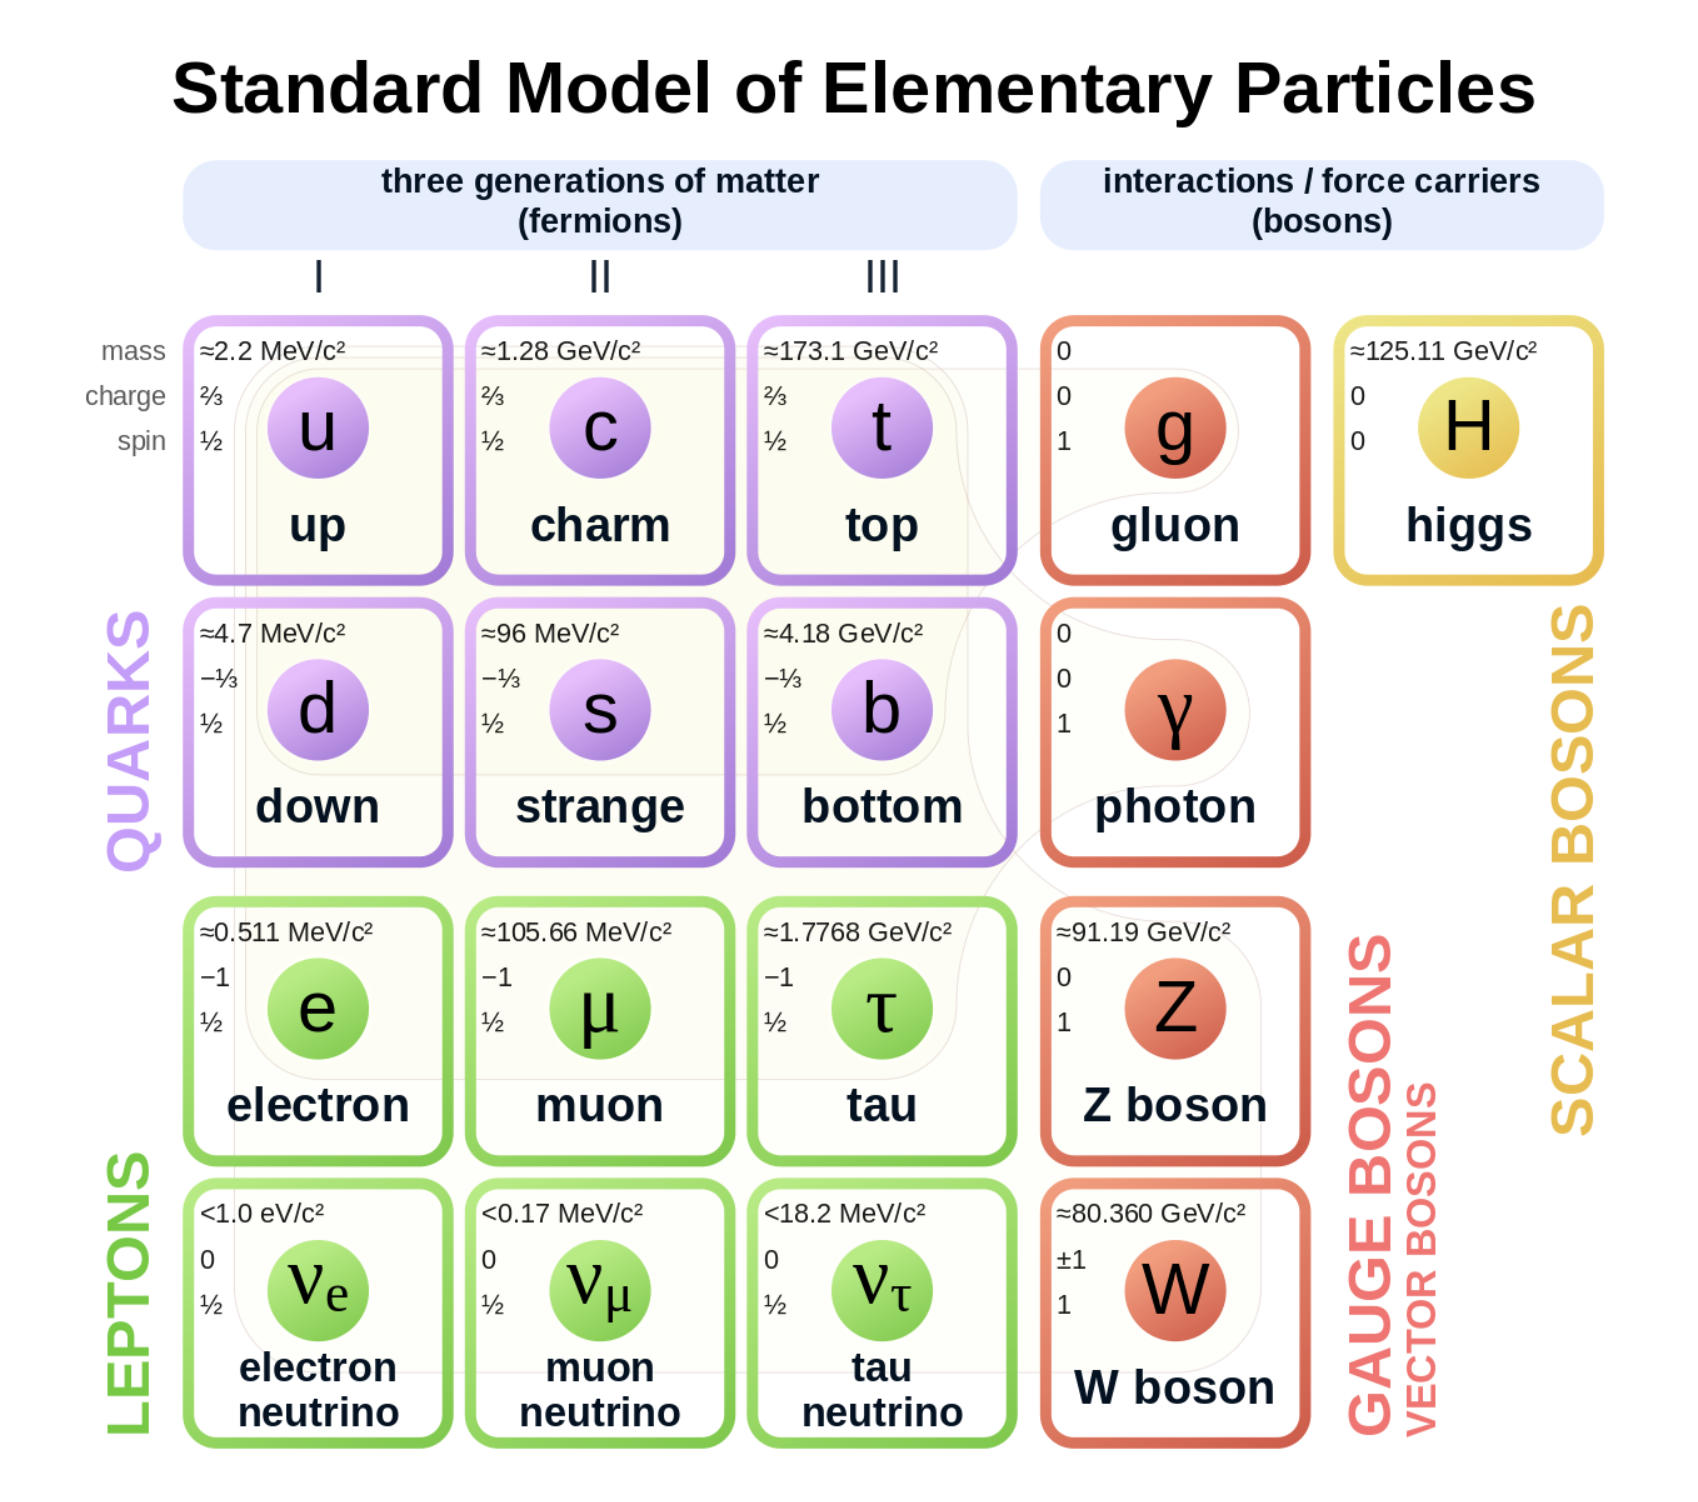
\includegraphics[width=0.7\textwidth]{figures/ch1/standard_model.png}
	\caption{Diagram of the 17 particles comprising the Standard Model}
	\label{fig:sm}
\end{figure}

Each entry is accompanied by 3 characteristic numbers: mass, charge, and spin. The mass of each particle is determined to limited precision by experimental observation, with the exception of photons and gluons which are known to be massless. Charge refers to the familiar electromagnetic charge in the case of leptons, W and Z bosons, and to color charge in the case of quarks and gluons. Spin is an intrinsic form of angular momentum carried by fundamental particles; all fermions have half integer spin, while bosons have integer spin. \par

Fermions come in flavor families
%flavors

Each particle is also known to have an \textit{antiparticle}. Each antiparticle has the same mass but the opposite charge of their Standard Model counter part; for example, the antiparticle of the electron is the positron, which has all the same properties but a positive charge. The photon, Z boson, and Higgs are all their own antiparticle. The nature of antineutrinos is an open question driving neutrino physics research, as it is not currently known whether neutrinos are their own antiparticle. \par

\subsection{Forces}
The three fundamental forces explained by the Standard Model are the electromagnetic force, the strong force, and the weak force. The photon is the carrier of the electromagnetic force, which dictates the nature of interactions between electrically charged particles, and is widely covered by introductory physics courses. The electromagnetic force has an infinite interaction range, a result of the massless and non-self interaction nature of the photon. The electromagnetic interaction is described by the theory of quantum electrodynamics (QED).\par

The weak force gives rise to atomic radiation and decay. It allows for the processes of beta decay and electron capture, which enable protons to convert to neutrons, and vice-versa, within the nucleus of an atom. In the process of beta decay, a proton decays into a neutron, a positron, and a neutrino; or, a neutron decays into a proton, an electron and an antineutrino. The weak interaction also plays a roll in the processes of nuclear fusion and nuclear fission. The  W\textsuperscript{+}, W\textsuperscript{-}, and Z\textsuperscript{0} are the force carriers of the weak force. The effective range of the weak force is limited to subatomic distances, as a result of the massive nature of the mediator bosons. The unified theory of the electroweak interaction posits that at high enough energies the electromagnetic interaction and the weak force merge into the same force. This threshold is termed the unification energy and estimated to be around 246 GeV. \par

The strong force confines quarks into hadron particles, such as protons and neutrons. The strong force also allows for the creation of atomic nuclei by binding protons and neutrons together, and is generally referred to as the ``nuclear force" in this context. The gluon is the mediator of the strong force, which is a short-range force which acts at subatomic distances on the order of $10^{-15}$ m. At this range, the strong force is about 100x as strong as the electromagnetic force, which allows for the creation of positively charged nuclei \cite{griffths}. The strong force is described by the theory of quantum chromodynamics (QCD). In the same way that QED dictates the interaction of electrically charges particles, QCD dictates the interactions of \textit{color-charged} particles. Due to the particular importance of QCD in this thesis, this topic will be explored in detail in section \ref{sec:QCD}. \par

The fundamental Feynmann diagram for each of the three forces discussed here is depicted in Figure \ref{fig:force_feynmann}. The fourth fundamental force, gravity, is not currently explained by any known mechanism within the Standard Model. 

 \begin{figure}
     \centering
     \begin{subfigure}[b]{0.43\textwidth}
         \centering
         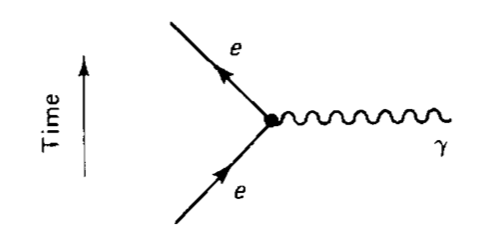
\includegraphics[width=\textwidth]{figures/ch1/em_force.png}
         \caption{The electromagnetic force}
     \end{subfigure}
     \hfill  
     \begin{subfigure}[b]{0.4\textwidth}
         \centering
         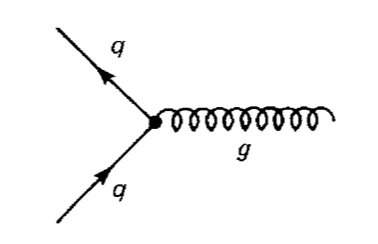
\includegraphics[width=\textwidth]{figures/ch1/strong_force.png}
         \caption{The strong force}
     \end{subfigure} \\
     \hfill
     \begin{subfigure}[b]{0.4\textwidth}
         \centering
         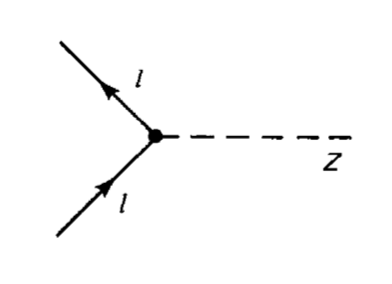
\includegraphics[width=\textwidth]{figures/ch1/weak_neutral.png}
         \caption{The neutral weak force}
     \end{subfigure}
     \hfill  
     \begin{subfigure}[b]{0.4\textwidth}
         \centering
         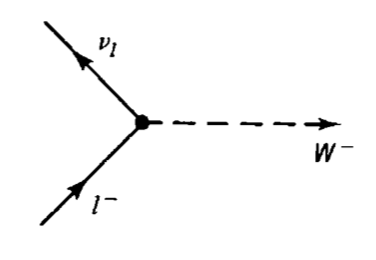
\includegraphics[width=\textwidth]{figures/ch1/weak_charged.png}
         \caption{The charged weak force}
     \end{subfigure} 
     \caption{Fundamental interactions of the three fundamental forces described by the Standard Model \cite{griffiths}. }
     \label{fig:force_feynmann}
\end{figure}

\section{QCD and Jets}
\label{sec:QCD}
The role of color in QCD at the surface level is analogous to that of electric charge in QED. However, while there is only one type of electric charge, there are three types of color charge - red, green, and blue. In the process $q \rightarrow q+g$, the color of the quark can change. In order to conserve color charge, gluons are bicolored, and always carry positive color charge and negative color charge. \par
Color charged particles only exist in bound states which result in a neutral total color charge, a principle known as confinement. This requires that quarks and gluons exist in group states known as hadrons; either mesons in the case of two quarks or baryons in the case of three quarks. When a quark is separated from a hadron, confinement dictates that other colored objects are produced around the quark to obey confinement. An example of this process is shown in Figure \ref{fig:jet_feynmann}. This ensemble of objects, generally a mixture of quarks and gluons, is termed a \textit{jet}. Jets are among the most common phenomenon observed by particle detectors at hadron colliders.

\begin{figure}
	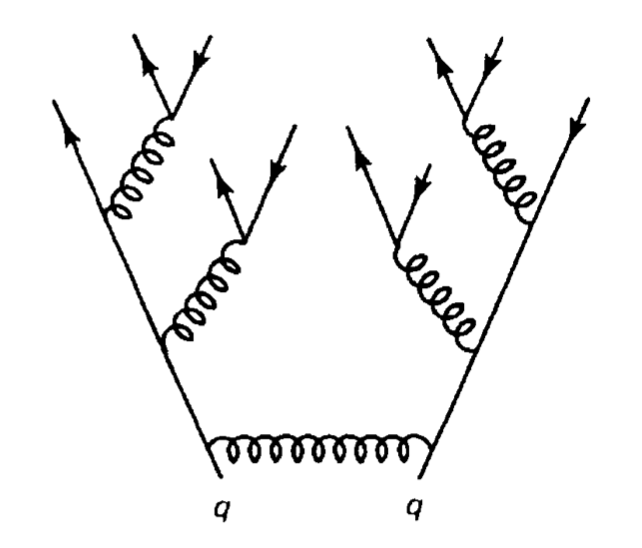
\includegraphics[width=0.5\textwidth]{figures/ch1/jet_feynmann.png}
	\caption{An example Feynmann diagram of jet production}
	\label{fig:jet_feynmann}
\end{figure}

\section{Symmetries}

The Standard Model is a renormalizable quantum field theory that obeys the local symmetry $G_{SM}$:

\begin{equation}
	G_{SM} = SU(3)_C \cross SU(2)_L \cross U(1)_Y .
\end{equation}

The $SU(3)_C$ symmetry component represents the non-Abelian gauge group of QCD. There are 8 generators for the $SU_C (3)$ group which correspond to the 8 types of gluon \cite{pdg}. \par

The $SU(2)_L \cross U(1)_Y$ symmetry group represents the electroweak sector of the Standard Model, which can be spontaneously broken into the electromagnetic and weak sectors. There are 4 generators for this group, which correspond to the four massless gauge bosons $W^1$, $W^2$, $W^3$, and B. From these massless gauge bosons are formed the massive mediators of the weak force, the $W^-$, $W^+$ and $Z^0$ bosons, and the massless electromagnetic force carrier, the photon $\gamma$. \par

Noether's theorem stipulates that any continuous symmetry is associated with a conserved quantity. In the Standard Model, this means that the $SU(3)_C$ symmetry gives rise to conservation of color charge. The $SU(2)_L \cross U(1)_Y$ symmetry gives rise to conservation of electromagnetic charge via symmetry breaking, which will be discussed in greater detail below. Conservation of spin results from the Poincar\'e symmetry described by the theory of special relativity, which combined with Noether's theorem gives us the conversation of energy, momentum, and angular momentum.\par

The SM Lagrangian is invariant under $CPT$ symmetry, or charge, parity, and time reversal. Charge conjugation ($C$) transform a particles into it's corresponding antipaticle by reversing the charge and other quantum numbers. Parity conjugation ($P$) reverses spatial coordinates, which transforms left-handed particles into right-handed particles and vice-versa. Time reversal ($T$) is the theoretical process of reversing time. The $L$ subscript in the $SU(2)_L$ group indicates that this symmetry only applies to the left-handed components of fermions. As a result, the $W^{1,2,3}$ generator bosons of $SU(2)_L$ only interact with left handed particles, a process which violates CP symmetry. The CPT theorem states that the violation of CP symmetry implies that T-symmetry must also be violated, so that $CPT$ is a preserved symmetry.

\subsection{Spontaneous Symmetry Breaking}
Higgs field a scalar field that forms a complex doublet of SU(2) 

Spontaneous symmetry breaking is the process by which a Lagranian obeys a symmetry at high energies, but exhibits asymmetric behavior at lower energies. The electroweak symmetry group is spontaneously broken as $SU(2)_L \cross U(1)_Y \rightarrow U(1)_{EM}$. The quantity conserved by the $SU(2)_L$ symmetry is weak isospin $T_{1,2,3}$, while the quantity conserved by $U(1)_Y$ symmetry is weak hypercharge $Y$. Below very high energies, the presence of the Higgs field causes the electroweak symmetry to break. This causes the four massless gauge bosons ($W^{1,2,3}$ and $B$) to mix, resulting in the massive gauge bosons $W^-$, $W^+$ and $Z^0$ bosons and the massless photon $\gamma$. The Higgs mechanism allows the $W^\pm$ and $Z$ bosons to be massive. The symmetry breaking also violates the conservation of weak isospin and weak hyperchage, leaving only electromagnetic charge $Q = T_3 + \frac{1}{2}Y$ as a conserved quantity associated with the $U(1)_{EM}$ symmetry. \par


\section{Experimental Validation of the Standard Model}
TODO: add citations for all original discoveries.\\

The theoretical framework of the Standard Model coalesced into a unified theory in the mid-20th century. A cascade of discoveries providing empirical evidence for the model followed closely. In the 1960s, three quarks (up, down and strange) and four leptons (electron, muon, and their associated neutrinos) were the known particulate building blocks of matter and the Standard Model. The discovery of the charm quark in 1974, through the observation of the $J/\psi$ meson \cite{SLAC_J}\cite{BNL_J}, confirmed the existence of a fourth quark flavor and explained the absence of flavor-changing neutral currents \cite{griffiths}. The discovery of the $\tau$ in 1975 \cite{tau} provided the first evidence of a 3rd generation of matter. This was quickly followed by the observation of the $\Upsilon$ meson in 1977, which provided evidence for the existence of a fifth quark, the $b$ bottom quark (sometimes also referred to as the beauty quark). The existence of a 3rd generation of fermion also explained the observation of CP violation in the weak force, as it allows for the appearance of a complex phase in the CKM matrix. The $t$ top quark and $\nu_\tau$ tau neutrino were predicted at this point as the final building blocks of three complete generations of fermions, and they were discovered by experimental observation around the turn of the 21st century. \par

The W and Z bosons were predicted by the Standard Model, but to observe them required the construction of a particle accelerator powerful enough to produce them. They were finally observed at CERN in 1983 by the UA1 and UA2 experiments at the newly constructed Super Proton Synchrotron (SPS). Their masses were observed to be compatible with those predicted by the Standard Model nearly a decade earlier. The final missing piece then was confirming the existence of the Higgs, which again required the construction of a newer and more powerful collider. CERN achieved this with the construction of the Large Hadron Collider (LHC), and in 2012 the ATLAS and CMS experiments announced the discovery of the Higgs particle. 

\section{Limitations of the Standard Model}
\label{sec:lim_sm}
TODO: add citations for all phenomenon.\\

While the Standard Model has enjoyed decades of experimental results which confirm its predictions, there are several glaring shortcomings. The observed phenomenon for which the Standard Model provides no explanation are summarized below.

\begin{itemize}
  \item Gravity - the Standard Model does not account for the fourth fundamental force of gravity.
  \item Dark Matter - there is no viable candidate to explain the existence of dark matter, a non-interacting form of matter which must exist to account for gravitational observations which cannot be explained by general relativity, such as the motion of galaxies, gravitational lensing, and the structure of the universe.
  \item Matter-Antimatter asymmetry - the level of CP violation in the Standard Model isn't sufficient to explain the large discrepancy between the amount of matter and the amount of antimatter in the universe today, and the origins of this imbalance are not understood.
  \item Neutrino masses - the Standard Model assumes that neutrinos are massless and provides no mechanism for them to acquire mass. However, observations of neutrino oscillations indicates they posses some very small but non-zero mass.
\end{itemize}

In additional to these unexplained natural phenomenon, there are several questions about the \textit{naturalness} of the Standard Model. The principle of naturalness states that dimensionless ratios between physical constants should be of order 1, and that nature should not be arbitrarily fine-tuned. While this is largely an aesthetic argument, it points to many aspects of the Standard Model for which there exists no natural explanation.

\begin{itemize}
  \item Strong CP - while CP symmetry is violated in the weak force, it appears to be preserved in the strong force, although CP violation in the strong force is allowed by the SM. There is no principle which motivates this incongruity between the weak force and strong force.
  \item Hierarchy Problem - The wide range of masses for elementary particles and the wide range of scales at which the four fundamental forces operate is not motivated by the SM. Specifically, it is not understood why the Higgs mass is observed to be well below the Plank scale $\lambda$, which is the energy level at which the effects of quantum gravity become significant. QFT indicates that the Higgs mass is determined by contributions from all energy scales including $\lambda$, which indicates that it's observed mass is inexplicably small.
\end{itemize}

These limitations of the Standard Model provide a road map for theoretical and experimental particle physicists, who seek to develop new theories which account for these observations, and then to find evidence which might support these \textit{beyond the Standard Model} (BSM) theories. The next chapter will introduce the BSM theories which motivate the physics search presented in this thesis. 
  
\chapter{Physics Beyond the Standard Model}
\section{Hidden Valley Theories}
\section{Semi-visible Jets}

%%%%%%%%%%%%%%%%
% Chapter 2
%%%%%%%%%%%%%%%%

\chapter{Physics Beyond the Standard Model}
In light of the various phenomenon unexplained by the Standard Model, physicists have proposed various extensions to the Standard Model, collectively termed \textit{Beyond the Standard Model} (BSM) theories. 
A particular focus of the physic programs at the Large Hadron Collider (LHC) are BSM models which suggest dark matter candidate particles. If these particles couple to Standard Model, they could be produced and observed at the LHC.

\section{Hidden Valley Models}
\label{sec:hiddenvalley}

Hidden Valley (HV) models are a category of BSM models that allow for dark matter (DM) production at the LHC. They extend the Standard Model with an additional non-Abelian gauge group \cite{snowmass}. This introduces the possibility of a complex dark sector, which mirrors the complexities of Standard Model QCD, and introduces the possibility of dark quarks and gluons. The term ``hidden valley" refers to the idea that the DM is hidden from the SM by a high-energy barrier, as illustrated in Figure \ref{fig:ch2/hidden_valley_sketch.png}. The dark sector is assumed to communicate with the Standard Model via a ``portal", or ``messenger particle", that can interact with both Standard Model and HV forces. For the s-channel scenario, the portal is considered to be a new massive mediator particle Z' . \par

\begin{figure}[h]
        \centering
	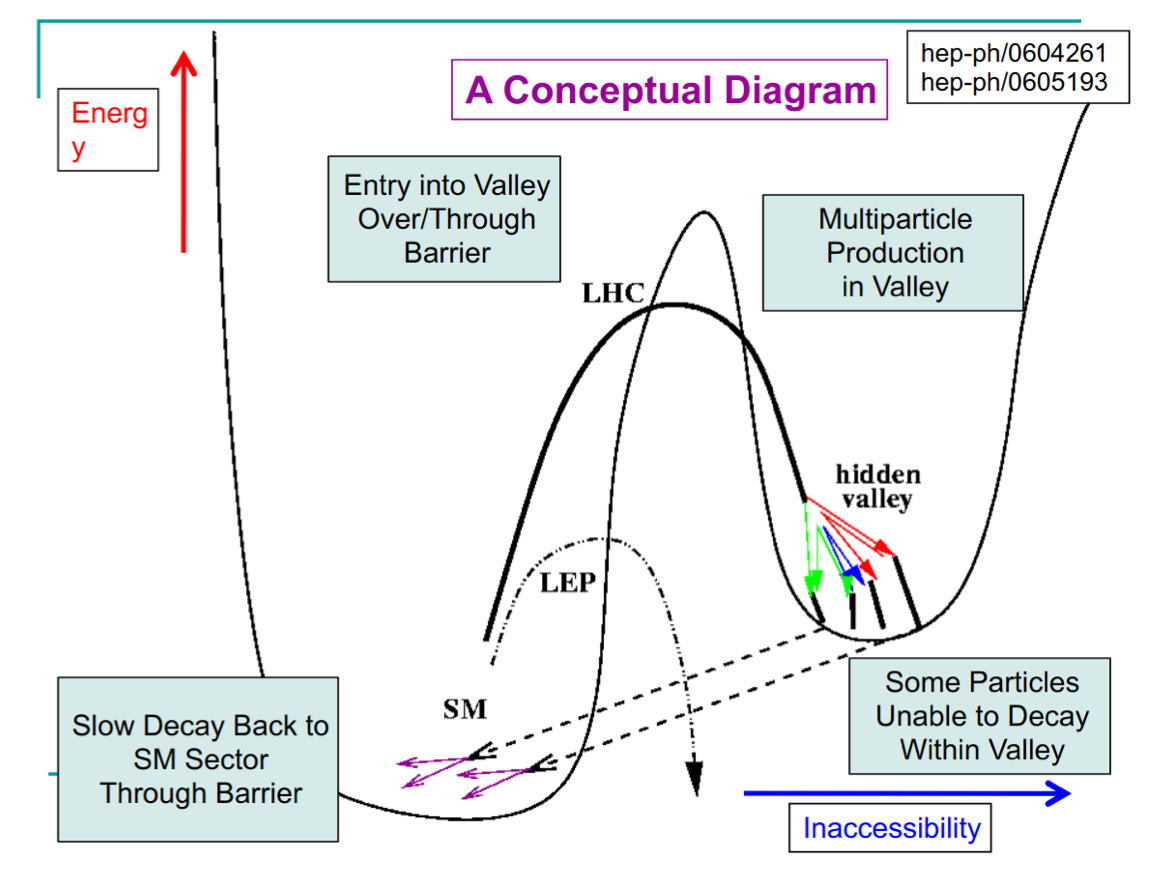
\includegraphics[width=.5\textwidth]{figures/ch2/hidden_valley_sketch.png}
        \label{fig:ch2/hidden_valley_sketch.png}
         \caption{Illustration of the hidden valley potential}
\end{figure}

The portal particle allows for the production of dark sector particles at hadron colliders. If dark quarks are produced via the decay $Z' \rightarrow q_D q_D$ they can hadronize and form dark jets. The properties of the dark jets are determined by the dynamics of the dark sector, which are explored in the subsequent section. Depending on the details of the model, the jets formed by the dark hadrons can be categorized as fully dark, semi-visible, leptonic, emerging, or other \cite{snowmass}. \par

\begin{figure}[h]
        \centering
	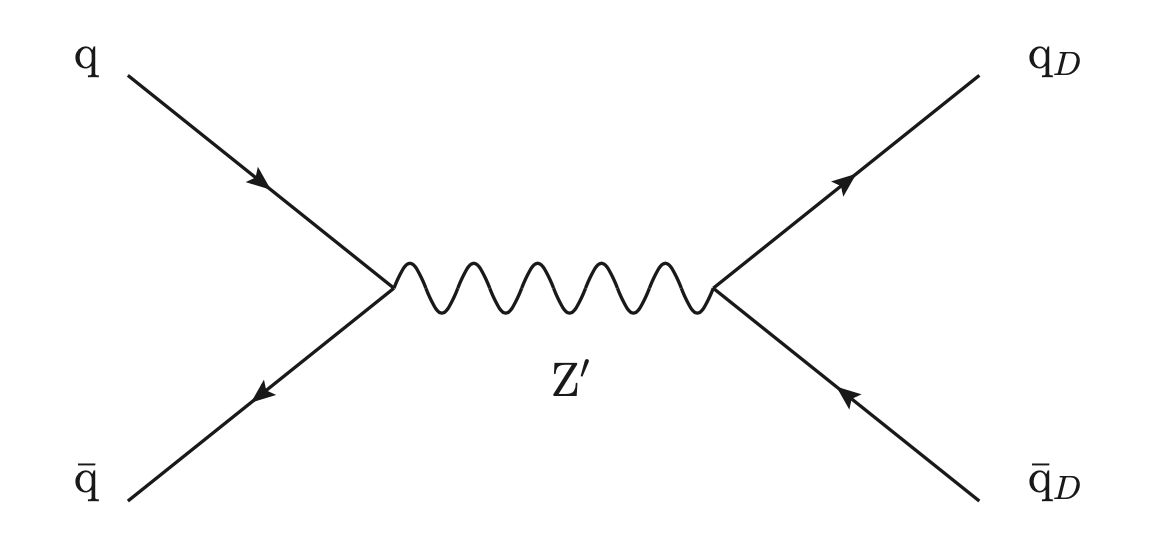
\includegraphics[width=.5\textwidth]{figures/ch2/zprime_feynman_diagram.png}
        \label{fig:ch2/zprime_feynman_diagram.png}
        \caption{The massive mediator particle Z' of the s-channel realization of a HV model}
\end{figure}

\section{Dark QCD}
\label{sec:darkqcd}
The theoretical underpinning of the semi-visible jet phenomenology is a dark sector with a gauge group $SU(N_d)$ leading to confinement at a scale $\Lambda_d$. For illustration, let's consider the case of an $SU(2)_d$ gauge theory, which gives rise to two dark fermionic generations $\chi_a = \chi_1, \chi_2$. Following the work of Timothy Cohen, et.al. we can write the fundamental dark Lagrangian as:
\begin{equation}
	\mathcal{L}_{dark} \supset - \frac{1}{2} \Tr G^{d}_{\mu\nu} G^{d\mu\nu} - \bar{\chi_a} (i {D\mkern-11.5mu/}-M_{d,a}) \chi_a
\end{equation}

The first term allows for the dark gluons to self-interact, while the second term enables the dark quarks to hadronize and acquire mass. The dark quarks are assumed to have a common mass $M_d$. The coupling strength of the strongly interacting dark quarks is termed $\alpha_d$. At the confinement scale $\Lambda_d$, the dark quarks can form bound states. At the scale $M_d \approx \Lambda_d$ a QCD-like show occurs. \par 

The properties of the hadrons formed by the dark quarks are of particular importance to the observed dark QCD dynamics. Dark-isospin number $U(1)_{1-2}$ and dark-baryon number $U(1)_{1+2}$ are accidental symmetries of the theory which determine the stability of the hadrons. In the case of two dark flavors, six dark hadrons can be formed: four mesons ($\chi_1\bar{\chi_1}$, $\chi_2\bar{\chi_2}$, $\chi_1\bar{\chi_2}$, $\bar{\chi_1}\chi_2$) and two baryons ($\bar{\chi_1}\bar{\chi_2}$, $\bar{\chi_1}\bar{\chi_2}$). The mesons $\chi_1\bar{\chi_2}$ and $\bar{\chi_1}\chi_2$ are charged under dark-isospin and will be stable if this symmetry is unbroken. The baryons would also be stable as they are charged under the dark-baryon number. These four stable hadrons become dark matter candidates of the theory. The $\chi_1\bar{\chi_1}$ and $\chi_2\bar{\chi_2}$ mesons are not charged under either symmetry and are thus expected to decay. The unstable mesons can decay into stable dark mesons, or into an off-shell Z'. The off-shell Z' will then decay into two DM quarks or two SM quarks, and it's products will continue to shower until the final state particles are stable.\par

The number of stable and unstable dark states varies substantially depending on the details of the model. The model discussed above can be generalized from $SU(2)_d$ to $SU(N)_d$, with any number of colors $N_c$ or flavors $N_f$. This affects the ratio of possible stable to unstable mesons, which can directly impact the amount of missing energy. The fraction of missing energy is a variable in many dark QCD models, and is especially important in the case of semi-visible jets.

\section{Semi-visible Jets}
\label{sec:semivisiblejets}

A ``semi-visible jet" occurs when the heavy Z' messenger particle decays into dark quarks, which then hadronize in a QCD-like shower. If some of the dark hadrons are stable while others decay to SM quarks via the off-shell Z', a collimated mixture of visible and dark matter is formed – this is termed a semi-visible jet. If the Z' messenger particle is produced at rest, the two jets will be back-to-back in the transverse plane. If there is an imbalance in the amount of invisible particles between the two jets, one of the jets will be observed to be aligned with missing transverse energy. \par

While there are a myriad of HV and dark QCD models, a handful of model parameters are most important in determining the observable of these showers within a particle detector. The coupling strength $\alpha_d$ is one of the most important, as it controls the fraction of dark hadrons emitted in the shower and their average \pt. The mass of the dark quarks directly impacts the jet mass. If the masses of the dark quark flavors are comparable, the ratio of stable to unstable dark hadrons will be approximately 1:1. However, if there is a mass splitting, stable or unstable dark hadrons may be favored, which impacts the amount of missing energy observed. \par

The ratio of stable to unstable dark hadrons in the shower is a critical variable for capturing the behavior of dark showers. This value is termed $r_{inv}$:
\begin{equation}
	r_{inv} = \frac{\textrm{\# of stable hadrons}}{\textrm{\# of hadronss}}
\end{equation}

Events containing jets aligned with missing transverse momentum are generally considered to be misreconstructed by other DM searches, and therefore discarded. This class of final states is therefore largely uncovered by existing DM searches. The nature of the dark hadron shower is determined by the following parameters: the Z' mass $m_{Z'}$, the Z' couplings to visible and dark quarks $g_q$ and $g_{q_D}$, the number of dark colors and flavors, the characteristic scale of the dark sector confinement $\Lambda_D$, the scale of the dark hadrons $m_D$, and the average fraction of stable hadrons in the decay $r_{inv}$. The coupling to SM quarks determines the Z' production cross section.



%%%%%%%%%%%%%%%%
% Chapter 3
%%%%%%%%%%%%%%%%

\chapter{The Large Hadron Collider}
The Large Hadron Collider (LHC) is a 26.7 km circular high-energy particle accelerator, spanning the Swiss-French border near the city of Geneva, Switzerland \cite{LHC_machine}. The LHC occupies the tunnel constructed in 1989 for the Large Electron-Positron (LEP) Collider, and reaches a maximum depth of 170m below the surface. The LHC is operated by the European Organization for Nuclear Research (CERN), the largest international scientific collaboration in the world.\par

The LHC accelerates protons and heavy ions, and collides them at four interaction points around the ring, with a design center-of-mass energy per collision of $\sqrt{s}$ = 14 TeV. Each interaction point is home to one of four detector experiments, which study the products of the collisions. The largest of these experiments is the ATLAS detector, a general purpose detector designed to study the Standard Model and search for new physics that could be produced in LHC collisions \cite{ATLAS_at_LHC}. The CMS detector is another general purpose detector, designed and operated independently of the ATLAS detector, but intended to probe the same range of physics \cite{CMS_at_LHC}. The ALICE experiment is a dedicated heavy ion experiment, and the LHC-b experiment is a dedicated $b$-physics experiment  \cite{ALICE_at_LHC} \cite{LHCb_at_LHC}.\par

This chapter will cover the multi-component accelerator complex powering the LHC, the state-of-the-art magnets which steer the particle beams, measurements of the intensity and number of collisions produced by the LHC, and finally an overview of LHC activities in the past, present, and future.

 \section{Accelerator Physics}
 \subsection{The Journey of a Proton}
 \label{sec:proton_journey}
From 2010 - 2018, the protons which fed the LHC started as hydrogen gas. The electrons were removed from the hydrogen atoms through the use of strong electric fields. The linear accelerator LINAC2 then accelerated the protons to an energy of 50 MeV. Between 2018 and 2020, LINAC2 was replaced with LINAC4, which instead accelerates $H^{-}$ ions, hydrogen atoms with two electrons. LINAC4 is capable of accelerating the $H^-$ ions to 160 MeV. Before injection to the next part of the acceleration chain, both electrons are stripped from the $H^-$ ions, leaving just protons. From here the protons enter the Proton Synchrotron booster, where they are accelerated up to 1.4 GeV of energy. Subsequently they are sorted into bunches separated in time by 25 ns, where each bunch contains approximately $10^{11}$ protons. Next the bunches pass through the Proton Synchrotron (PS) and the Super Proton Synchrotron (SPS), where they reach energies of 25 GeV and 450 GeV respectively. Finally they are injected into the LHC as two beams traveling in opposite direction. The original design allowed each beam to be accelerated up to 7 TeV of energy. Due to limitations in the performance of the superconducting LHC magnets, the highest energy actually achieved by the LHC beams during Run 2 was 6.5 TeV, giving a collision center-of-mass energy of $\sqrt{s}$ = 13 TeV \cite{lhc_faq}. Figure \ref{fig:accelerator_complex} shows the full LHC accelerator complex.\par

\begin{figure}
	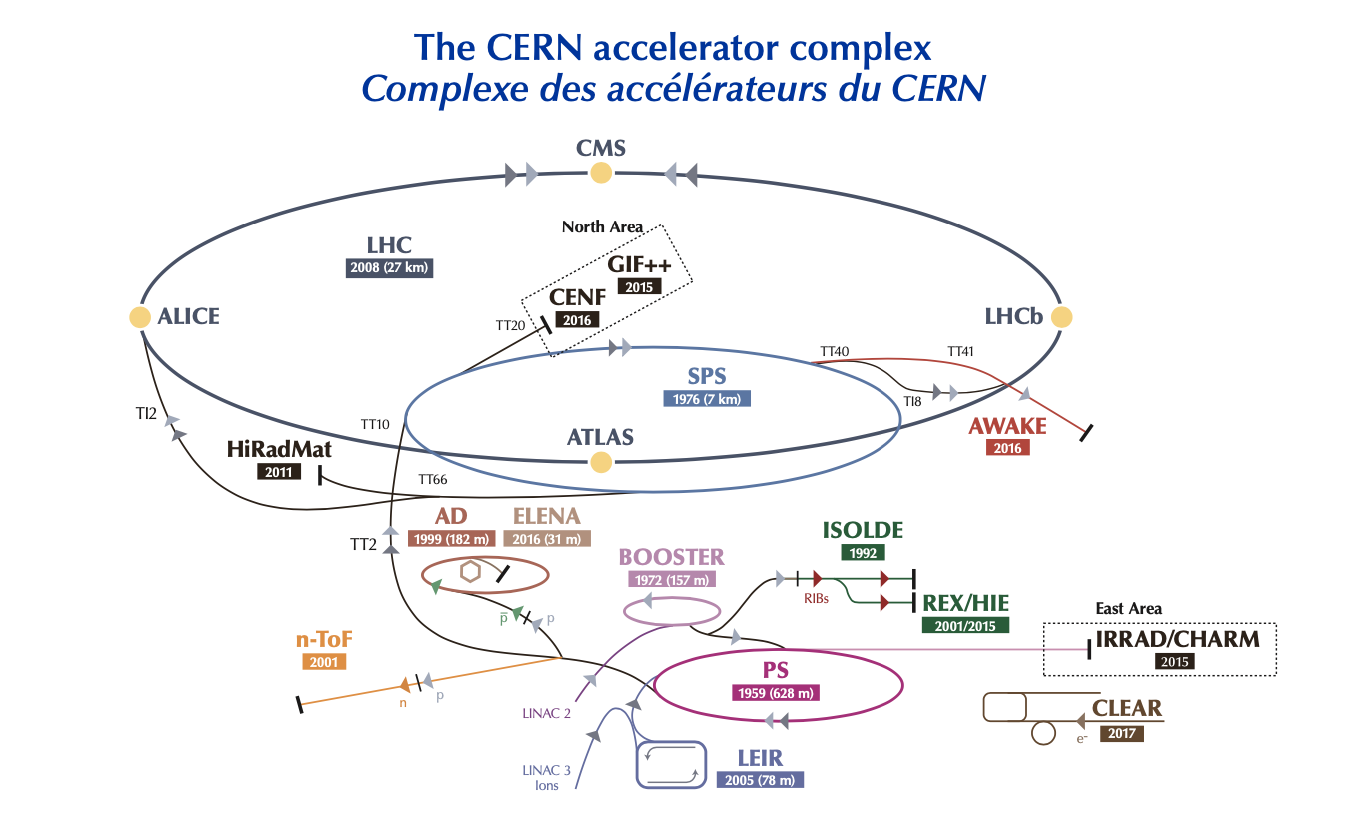
\includegraphics[width=\textwidth]{figures/ch3/accelerator_complex.png}
	\caption{The LHC accelerator complex at CERN \cite{cern_accelerator_complex}}
	\label{fig:accelerator_complex}
\end{figure}

 Acceleration in the LHC is performed by eight radio frequency (RF) cavities located around the ring. Each RF cavity produces a 2 MV electric field oscillating at 40 MHz. The 40MHz oscillation produces a point of stable equilibrium every 2.5 ns. These points of equilibrium are synchronized with the occurrence of the proton bunches produced in the PS -- a proton bunch occupies one out of every ten points of stable equilibrium, such that the bunches maintain a 25 ns spacing \cite{lhc_faq}. \\

\subsection{Magnets}
In addition to the acceleration cavities, the LHC houses 9593 superconducting magnets which direct and focus the proton beam on its 27 kilometer journey. The magnets are comprised of superconducting Niobium-Titanium coils cooled to 1.9K by superfluid helium. As the beams approach one of the four collision points around the ring, multipole magnets focus and squeeze the beam for optimal collisions \cite{lhc_faq}.\par

The LHC is divided into sections, where each section contains an a smoothly curving \textit{arc} and a straight \textit{insertion}. The arcs are composed of 1232 large dipole magnets which bend the beam to follow the roughly circular 27 km path. The main dipoles generate powerful 8.3 tesla magnetic fields to achieve this bend. Each dipole magnet is 15 meters long and weighs 35 tonnes. The dipoles work in conjunction with quadrupole magnets, which keep the particles in a focused beam, and smaller sextupole, octupole and decapole magnets which tune the magnetic field at the ends of the dipole magnets \cite{lhc_magnets}.\par

The straight insertion sections have different purposes depending on their location around the ring: beam collisions, beam injection, beam dumping, or beam cleaning. At the four collision points, insertion magnets squeeze the beam to ensure a highly focused collision. This is accomplished with a triplet of quadrupole magnets, which tighten the beam from 0.2 millimeters to just 16 micrometers in diameter. Insertion magnets also clean the beam, which prevents stray particles from hitting sensitive components throughout the LHC. When the LHC is ready to dispose of a beam of particles, beam dump magnets deflect the path of the beam into a straight line towards a block of concrete and graphite that stops the beam. A dilution magnet then reduces the beam intensity by a factor of 100,000 before the final stop \cite{lhc_magnets}. Figure \ref{fig:lhc_octants} shows the locations various beam activities.\par

\begin{figure}
        \centering
	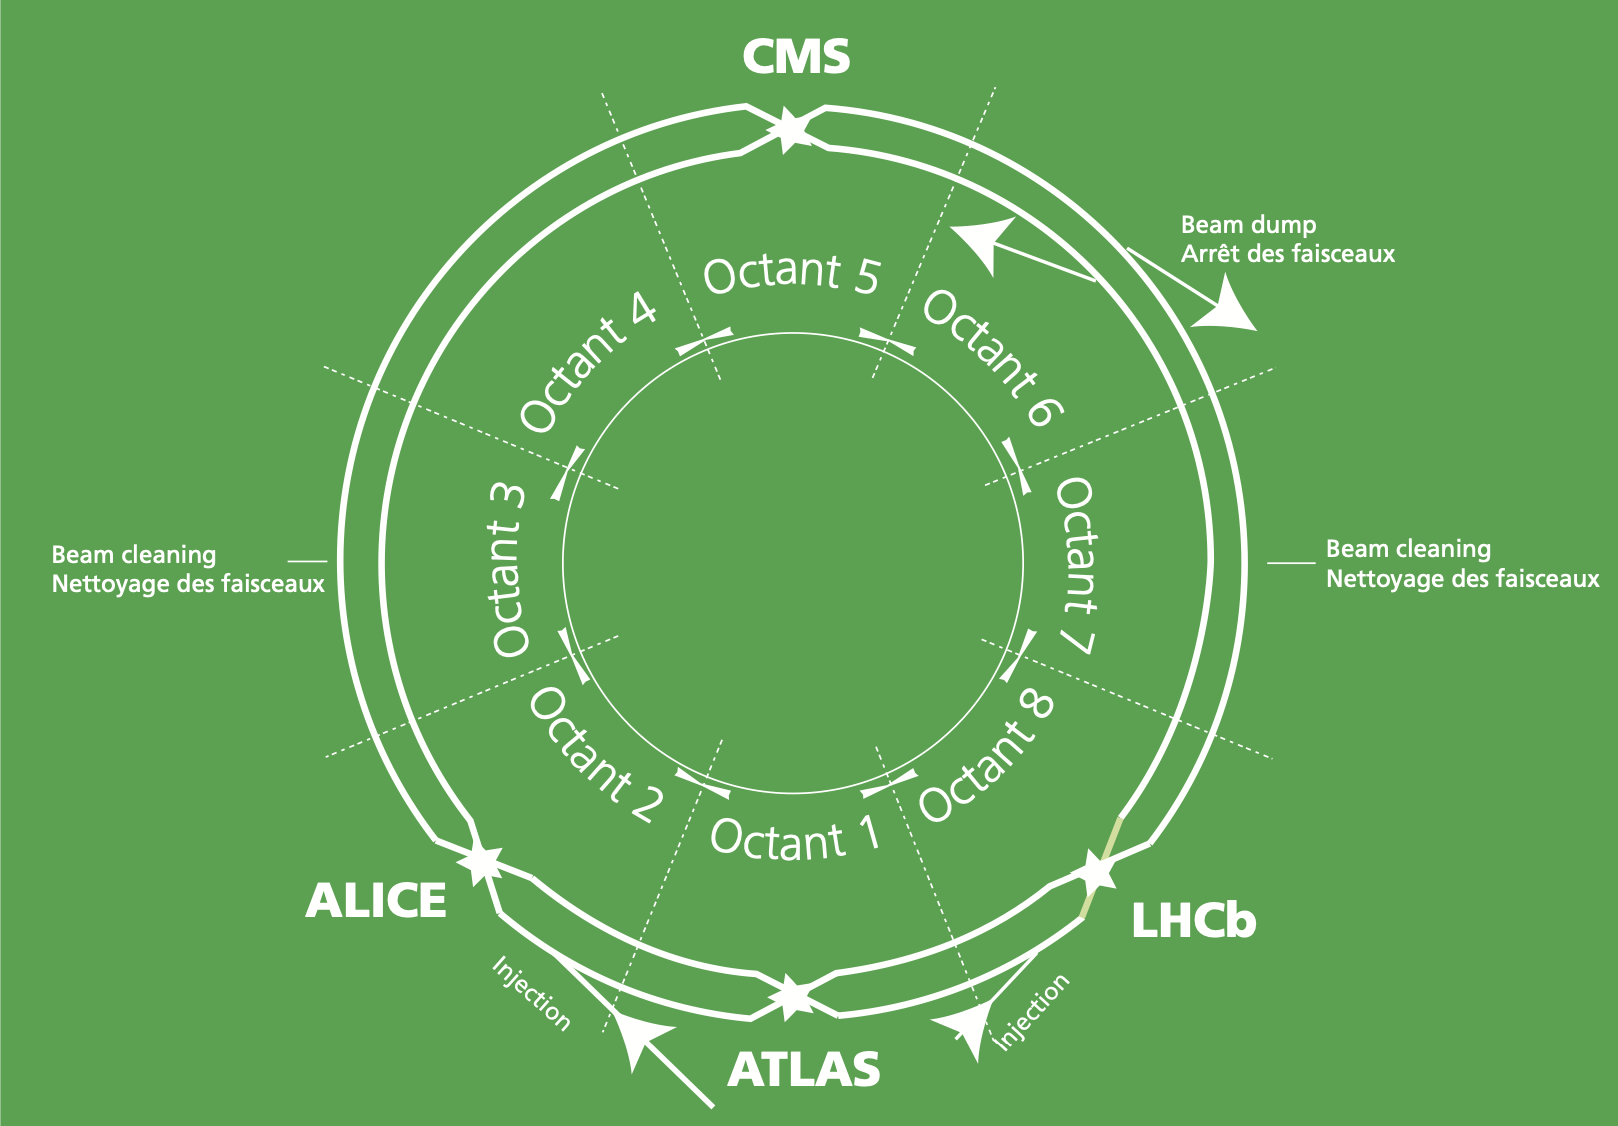
\includegraphics[width=.7\textwidth]{figures/ch3/lhc_octants.png}
	\caption{The octants of the LHC and location of various beam activities \cite{lhc_faq}. Stars indicate the locations of beam collisions, and the associated detectors recording the outcome of those collisions.}
	\label{fig:lhc_octants}
\end{figure} 
 
 \section{Luminosity}
 
Collisions at the LHC occur when the two beams of proton bunches cross at one of the four interaction points. The intensity of collisions is described by the instantaneous luminosity, the formula for which is given in equation \ref{eq:lumi}.  
 \begin{equation}
	L = \frac{f N_1 N_2}{4 \pi \sigma_x \sigma_y}
	\label{eq:lumi}
\end{equation}

Here $f$ is the revolution frequency, $N_1$ and $N_2$ are the number of particle per bunch for each beam, and $\sigma_x$, $\sigma_y$ are the horizontal and vertical beam widths. \par

The instantaneous luminosity gives the number of the collisions that could be produced at the interaction point per unit of cross-sectional area per unit of time, generally expressed in cm\textsuperscript{-2}s\textsuperscript{-1}. The integrated luminosity is obtained by integrating the instantaneous luminosity over a given block of time, and measures the total number of collisions which have occurred during that operation period. The total integrated luminosity is directly correlated with the size of the datasets collected by the LHC experiments. Total integrated luminosity for Run 2 is illustrated in Figure \ref{fig:lumi_run2}. \par 

High levels of instantaneous luminosity result in multiple $pp$ collisions per bunch crossing, which leads to an effect known as $pileup$. Pileup poses a challenge for detector physics, as reconstructing the products of multiple simultaneous events is far more challenging than reconstructing a single event with no pileup. Pileup conditions vary from year-to-year and run-to-run of LHC operation, and the impact of these conditions are taken into account when analyzing the data, as will be discussed further in Chapter \ref{ch:part_reco}. Measurement of pileup conditions during Run 2 are illustrated in Figure \ref{fig:lumi_run2}. \par
 
 \begin{figure}
     \centering
     \begin{subfigure}[b]{0.49\textwidth}
         \centering
         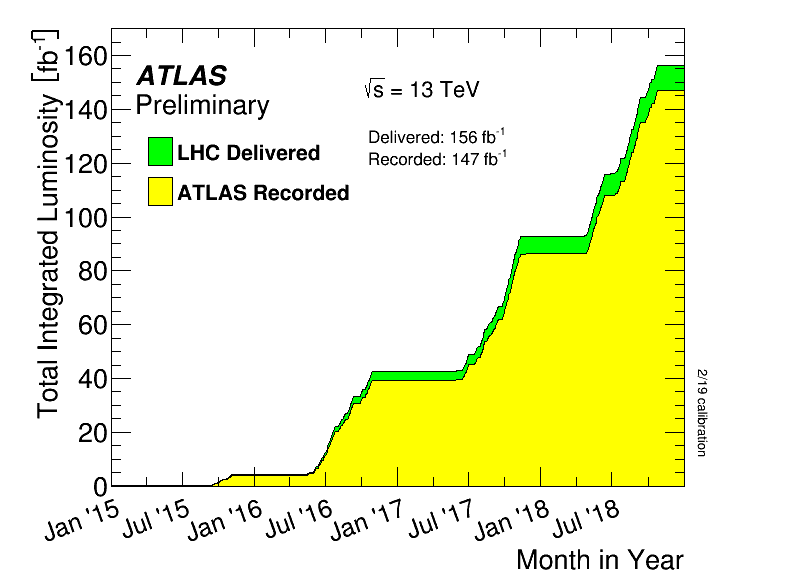
\includegraphics[width=\textwidth]{figures/ch3/lumi_integrated.png}
     \end{subfigure}
     \hfill  
     \begin{subfigure}[b]{0.48\textwidth}
         \centering
         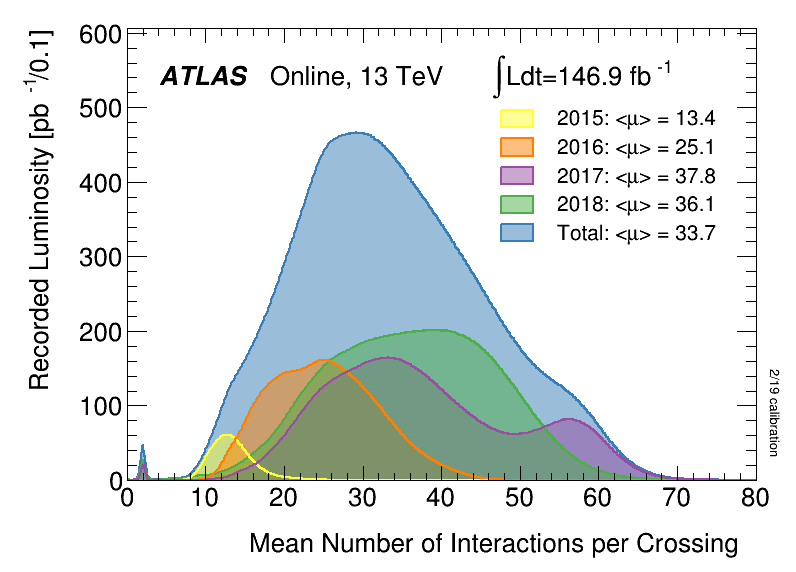
\includegraphics[width=\textwidth]{figures/ch3/lumi_instantaneous.png}
     \end{subfigure}
     \hfill
     \caption { (Left) Total integrated luminosity over the course of Run 2. (Right) Average number of $pp$ interactions per bunch crossing in Run 2. Each curve is weighted by the integrated luminosity for the year.}
     \label{fig:lumi_run2}
\end{figure}
 
 The design peak luminosity of the LHC is $1.0 \times 10^{34}$ cm\textsuperscript{-2}s\textsuperscript{-1}. During Run 1 of the LHC the peak instantaneous luminosity was $0.8 \times 10^{34}$ cm\textsuperscript{-2}s\textsuperscript{-1}. Over the course of Run 1 the LHC collected a total integrated luminosity of 5.46 \invfb at $\sqrt{s} = 7$ TeV, and 22.8 \invfb at $\sqrt{s} = 8$ TeV. Following the first long shutdown and upgrade phase of operations, the LHC achieved a center of mass energy $\sqrt{s} = 13$ TeV at the beginning of Run 2 in 2015. The LHC was also able to deliver $2.0 \times 10^{34}$ cm\textsuperscript{-2}s\textsuperscript{-1} peak instantaneous luminosity, double the design value. During LHC Run 2, from 2015-2018, the LHC delivered 156 \invfb of integrated luminosity for proton-proton collisions. Run 3 of the LHC began in 2022, and is expected to deliver $250$ \invfb of integrated luminosity to the ATLAS and CMS experiments by 2026 \cite{lhc_timeline}.\par
 
The goal of LHC physic analyses is to find and study rare events produced by interesting physics processes. The cross section $\sigma$ of a given process indicates the probability of that process occurring given the beam conditions of the LHC. Multiplying the cross section by the integrated luminosity of a dataset gives the expected number of events for that process within the dataset.

 \begin{equation}
	N\textsubscript{events} = \int \sigma L(t) dt = \mathcal{L} \times \sigma
	\label{eq:xs}
\end{equation}

The cross section for most processes of interest, especially BSM processes, is several orders of magnitude below the total cross section for the LHC. Therefore maximizing the number of events produced in collisions is crucial to increase the likelihood of producing events from processes of interest. For this reason, maximizing instantaneous luminosity is a key factor in accelerator design and operation, while mitigating the resulting pileup effects is a key component in detector design and operation. \par 

\section{LHC Timeline}
The first proton-proton collisions at the LHC were achieved in 2010 with a center-of-mass energy of $\sqrt{s}$ = 7 TeV. Run 1 of the LHC took place between 2010 and early 2013, during which time the center-of-mass collision energy increased from 7 TeV to 8 TeV. Figure \ref{fig:lhc_timeline} shows an overview of LHC activities beginning in 2011, in the midst of Run 1. The data collected during Run 1 led to the discovery of the Higgs boson in 2012 \cite{higgs_paper}. \par

Between 2013 and 2015 the LHC underwent the first Long Shutdown (LS1) during which time maintenance and renovation was performed on the accelerator chain, including the repair and consolidation of the high-current splices which connect the super-conducting LHC magnets. Run 2 of the LHC took place from 2015 to 2018 and achieved a center-of-mass energy of $\sqrt{s}$ = 13 TeV. Analysis of data collected in Run 2 is still on going, and is the subject of study in this thesis. \par

Between 2018 and 2022 the LHC underwent the second Long Shutdown (LS2), allowing for further detector and accelerator maintenance and upgrades. Key improvements to the LHC included the improvement of the insulation for over 1200 diode magnets, and the upgrade from LINAC2 to LINAC4 mentioned in Section \ref{sec:proton_journey}. Run 3 of the LHC began in 2022 and achieved a center-of-mass energy of $\sqrt{s}$ = 13.6 TeV. \par

Run 3 is scheduled to continue through 2026, at which point the LHC machine and detectors will undergo upgrades for the \textit{high luminosity} LHC (HL-LHC). The HL-LHC will increase the instantaneous machine luminosity by a factor of 5 - 7.5 with respect to the nominal LHC design. The bottom panel of Figure \ref{fig:lhc_timeline} shows an overview of the preparation work for the HL-LHC that has been going on concurrently with Run 1, 2, and 3 of the LHC \cite{hl_lhc}. 

\begin{figure}
        \centering
	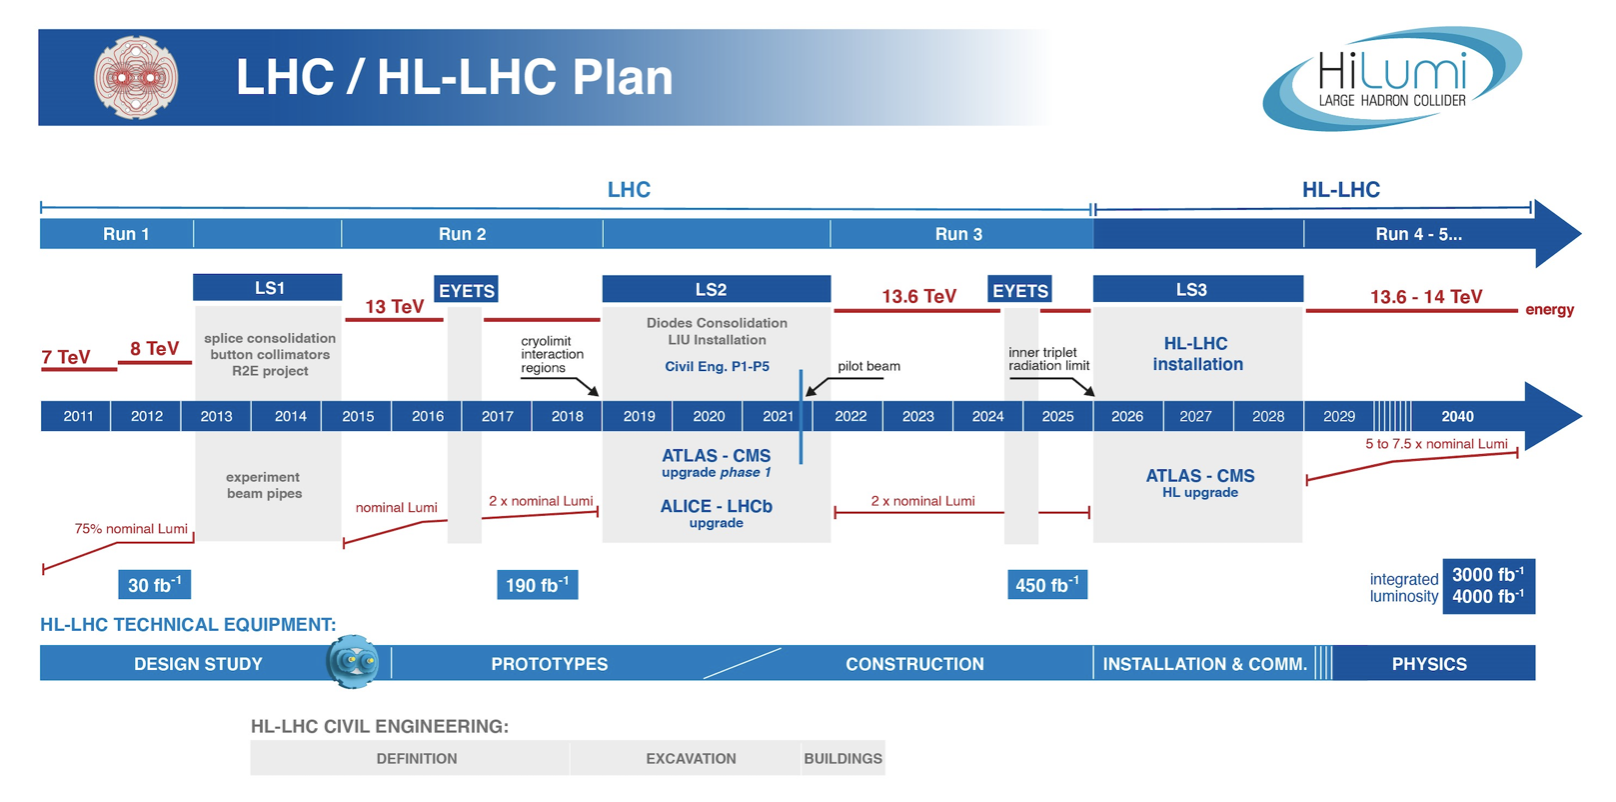
\includegraphics[width=0.9\textwidth]{figures/ch3/hl_lhc_timeline.png}
	\caption{Timeline of LHC and HL-LHC activities \cite{lhc_timeline}. Integrated luminosity estimates are approximate, and not reflective of the exact amount delivered to each experiment.}
	\label{fig:lhc_timeline}
\end{figure}



%%%%%%%%%%%%%%%%
% Conclusion
%%%%%%%%%%%%%%%%


\clearpage
\phantomsection
\addcontentsline{toc}{chapter}{Conclusion or Epilogue}

\begin{center}
\pagebreak
\vspace*{5\baselineskip}
\textbf{\large Conclusion or Epilogue}
\end{center}


\begin{flushleft}
\hspace{10mm}Use this page for your epilogue or conclusion if applicable; please use only one of the titles for this page. Otherwise, you may delete it.
Use this page for your epilogue or conclusion if applicable; please use only one of the titles for this page. Otherwise, you may delete it.
Use this page for your epilogue or conclusion if applicable; please use only one of the titles for this page. Otherwise, you may delete it.
Use this page for your epilogue or conclusion if applicable; please use only one of the titles for this page. Otherwise, you may delete it.
Use this page for your epilogue or conclusion if applicable; please use only one of the titles for this page. Otherwise, you may delete it.
Use this page for your epilogue or conclusion if applicable; please use only one of the titles for this page. Otherwise, you may delete it.
Use this page for your epilogue or conclusion if applicable; please use only one of the titles for this page. Otherwise, you may delete it.
Use this page for your epilogue or conclusion if applicable; please use only one of the titles for this page. Otherwise, you may delete it.
Use this page for your epilogue or conclusion if applicable; please use only one of the titles for this page. Otherwise, you may delete it.Use this page for your epilogue or conclusion if applicable; please use only one of the titles for this page. Otherwise, you may delete it.Use this page for your epilogue or conclusion if applicable; please use only one of the titles for this page. Otherwise, you may delete it.
Use this page for your epilogue or conclusion if applicable; please use only one of the titles for this page. Otherwise, you may delete it.Use this page for your epilogue or conclusion if applicable; please use only one of the titles for this page. Otherwise, you may delete it.
Use this page for your epilogue or conclusion if applicable; please use only one of the titles for this page. Otherwise, you may delete it.
Use this page for your epilogue or conclusion if applicable; please use only one of the titles for this page. Otherwise, you may delete it.
Use this page for your epilogue or conclusion if applicable; please use only one of the titles for this page. Otherwise, you may delete it.
Use this page for your epilogue or conclusion if applicable; please use only one of the titles for this page. Otherwise, you may delete it.
Use this page for your epilogue or conclusion if applicable; please use only one of the titles for this page. Otherwise, you may delete it.
Use this page for your epilogue or conclusion if applicable; please use only one of the titles for this page. Otherwise, you may delete it.
Use this page for your epilogue or conclusion if applicable; please use only one of the titles for this page. Otherwise, you may delete it.
Use this page for your epilogue or conclusion if applicable; please use only one of the titles for this page. Otherwise, you may delete it.
Use this page for your epilogue or conclusion if applicable; please use only one of the titles for this page. Otherwise, you may delete it.
Use this page for your epilogue or conclusion if applicable; please use only one of the titles for this page. Otherwise, you may delete it.Use this page for your epilogue or conclusion if applicable; please use only one of the titles for this page. Otherwise, you may delete it.Use this page for your epilogue or conclusion if applicable; please use only one of the titles for this page. Otherwise, you may delete it.
Use this page for your epilogue or conclusion if applicable; please use only one of the titles for this page. Otherwise, you may delete it.Use this page for your epilogue or conclusion if applicable; please use only one of the titles for this page. Otherwise, you may delete it.
Use this page for your epilogue or conclusion if applicable; please use only one of the titles for this page. Otherwise, you may delete it.
Use this page for your epilogue or conclusion if applicable; please use only one of the titles for this page. Otherwise, you may delete it.
Use this page for your epilogue or conclusion if applicable; please use only one of the titles for this page. Otherwise, you may delete it.
Use this page for your epilogue or conclusion if applicable; please use only one of the titles for this page. Otherwise, you may delete it.
Use this page for your epilogue or conclusion if applicable; please use only one of the titles for this page. Otherwise, you may delete it.
Use this page for your epilogue or conclusion if applicable; please use only one of the titles for this page. Otherwise, you may delete it.
Use this page for your epilogue or conclusion if applicable; please use only one of the titles for this page. Otherwise, you may delete it.
Use this page for your epilogue or conclusion if applicable; please use only one of the titles for this page. Otherwise, you may delete it.
Use this page for your epilogue or conclusion if applicable; please use only one of the titles for this page. Otherwise, you may delete it.
Use this page for your epilogue or conclusion if applicable; please use only one of the titles for this page. Otherwise, you may delete it.Use this page for your epilogue or conclusion if applicable; please use only one of the titles for this page. Otherwise, you may delete it.Use this page for your epilogue or conclusion if applicable; please use only one of the titles for this page. Otherwise, you may delete it.
Use this page for your epilogue or conclusion if applicable; please use only one of the titles for this page. Otherwise, you may delete it.Use this page for your epilogue or conclusion if applicable; please use only one of the titles for this page. Otherwise, you may delete it.
Use this page for your epilogue or conclusion if applicable; please use only one of the titles for this page. Otherwise, you may delete it.
Use this page for your epilogue or conclusion if applicable; please use only one of the titles for this page. Otherwise, you may delete it.
Use this page for your epilogue or conclusion if applicable; please use only one of the titles for this page. Otherwise, you may delete it.
Use this page for your epilogue or conclusion if applicable; please use only one of the titles for this page. Otherwise, you may delete it.
Use this page for your epilogue or conclusion if applicable; please use only one of the titles for this page. Otherwise, you may delete it.
Use this page for your epilogue or conclusion if applicable; please use only one of the titles for this page. Otherwise, you may delete it.
Use this page for your epilogue or conclusion if applicable; please use only one of the titles for this page. Otherwise, you may delete it.
Use this page for your epilogue or conclusion if applicable; please use only one of the titles for this page. Otherwise, you may delete it.
Use this page for your epilogue or conclusion if applicable; please use only one of the titles for this page. Otherwise, you may delete it.
Use this page for your epilogue or conclusion if applicable; please use only one of the titles for this page. Otherwise, you may delete it.Use this page for your epilogue or conclusion if applicable; please use only one of the titles for this page. Otherwise, you may delete it.Use this page for your epilogue or conclusion if applicable; please use only one of the titles for this page. Otherwise, you may delete it.
Use this page for your epilogue or conclusion if applicable; please use only one of the titles for this page. Otherwise, you may delete it.Use this page for your epilogue or conclusion if applicable; please use only one of the titles for this page. Otherwise, you may delete it.
Use this page for your epilogue or conclusion if applicable; please use only one of the titles for this page. Otherwise, you may delete it.
Use this page for your epilogue or conclusion if applicable; please use only one of the titles for this page. Otherwise, you may delete it.
Use this page for your epilogue or conclusion if applicable; please use only one of the titles for this page. Otherwise, you may delete it.
Use this page for your epilogue or conclusion if applicable; please use only one of the titles for this page. Otherwise, you may delete it.
Use this page for your epilogue or conclusion if applicable; please use only one of the titles for this page. Otherwise, you may delete it.
Use this page for your epilogue or conclusion if applicable; please use only one of the titles for this page. Otherwise, you may delete it.
Use this page for your epilogue or conclusion if applicable; please use only one of the titles for this page. Otherwise, you may delete it.
Use this page for your epilogue or conclusion if applicable; please use only one of the titles for this page. Otherwise, you may delete it.
Use this page for your epilogue or conclusion if applicable; please use only one of the titles for this page. Otherwise, you may delete it.
Use this page for your epilogue or conclusion if applicable; please use only one of the titles for this page. Otherwise, you may delete it.Use this page for your epilogue or conclusion if applicable; please use only one of the titles for this page. Otherwise, you may delete it.Use this page for your epilogue or conclusion if applicable; please use only one of the titles for this page. Otherwise, you may delete it.
Use this page for your epilogue or conclusion if applicable; please use only one of the titles for this page. Otherwise, you may delete it.Use this page for your epilogue or conclusion if applicable; please use only one of the titles for this page. Otherwise, you may delete it.
Use this page for your epilogue or conclusion if applicable; please use only one of the titles for this page. Otherwise, you may delete it.
\end{flushleft}


%\pagenumbering{gobble}  %remove page number on summary page





%%%%%%%%%%%%%%%%
% References
%%%%%%%%%%%%%%%%
\clearpage
\phantomsection 
\titleformat{\chapter}[display]
{\normalfont\bfseries\filcenter}{}{0pt}{\large\bfseries\filcenter{#1}}  % Reset title format for Reference section. (It is different from Chapter titles)
\titlespacing*{\chapter}
  {0pt}{0pt}{30pt}

\begin{singlespace}  % use single-line spacing for multi-line text within a single reference
	\setlength\bibitemsep{\baselineskip}  %manually set separataion betwen items in bibliography to double space
	\addcontentsline{toc}{chapter}{References}  %add References section to Table of Contents
	\printbibliography[title={References}]
\end{singlespace}



%%%%%%%%%%%%%%%%
% Appendices
%%%%%%%%%%%%%%%%

%Readjust Title format for Appendicies
\titleformat{\chapter}[display]
{\normalfont\bfseries\filcenter}{}{0pt}{\large\chaptertitlename\ \large\thechapter : \large\bfseries\filcenter{#1}}  
\titlespacing*{\chapter}
  {0pt}{0pt}{30pt}	%controls vertical margins on title
  
% Adjust section title formatting
\titleformat{\section}{\normalfont\bfseries}{\thesection}{1em}{#1}

% Adjust subsection title formatting
\titleformat{\subsection}{\normalfont}{\thesubsection}{0em}{\hspace{1em}#1}

\begin{appendices}

%Some Table of Contents entry formatting
\addtocontents{toc}{\protect\renewcommand{\protect\cftchappresnum}{\appendixname\space}}
\addtocontents{toc}{\protect\renewcommand{\protect\cftchapnumwidth}{6em}}

%Begin individual appendices, separated as chapters

\chapter{ Experimental Equipment}
Lorem ipsum dolor sit amet, consectetur adipiscing elit, sed do eiusmod tempor incididunt ut labore et dolore magna aliqua. Ut enim ad minim veniam, quis nostrud exercitation ullamco laboris nisi ut aliquip ex ea commodo consequat. Duis aute irure dolor in reprehenderit in voluptate velit esse cillum dolore eu fugiat nulla pariatur. Excepteur sint occaecat cupidatat non proident, sunt in culpa qui officia deserunt mollit anim id est laborum.

\chapter{Data Processing}
Lorem ipsum dolor sit amet, consectetur adipiscing elit, sed do eiusmod tempor incididunt ut labore et dolore magna aliqua. Ut enim ad minim veniam, quis nostrud exercitation ullamco laboris nisi ut aliquip ex ea commodo consequat. Duis aute irure dolor in reprehenderit in voluptate velit esse cillum dolore eu fugiat nulla pariatur. Excepteur sint occaecat cupidatat non proident, sunt in culpa qui officia deserunt mollit anim id est laborum.

\end{appendices}

\end{document} 
